% Close the paper, review what you did, and close things up.

% Where the abstract is usually a section telling us what you did and a ``teaser'' of the results, a conclusion would instead remind us of all of what you covered.
% You can think of a conclusion as a ``retrospective abstract.''

% conclusion.tex
% \section{Conclusion}
% Our systematic evaluation shows that Scrapy, by default, offers no defenses against SQL Injection, Cross‐Site Scripting, or malicious file downloads. Crawler pipelines assume benign inputs: form payloads are unsanitized, event‐handlers execute unfiltered in a headless browser, and binaries are retrieved without scanning. To safely deploy Scrapy in adversarial settings, practitioners must layer in input validation, response‐pattern analysis, Content Security Policy enforcement, and sandboxed execution environments. Our ScrapyShield framework provides a reusable test harness to guide future hardening efforts and underscores the need for a security-first mindset when building web‐scale automation.

\section{Results}

\subsection{SQL Injection Results}
To evaluate Scrapy’s behavior when encountering SQL Injection (SQLi) attack vectors, we developed a spider targeting a deliberately vulnerable login page (\texttt{/sqli}) hosted on the malicious Flask server. The login form failed to sanitize inputs, creating an ideal scenario for SQL Injection testing. Our objective was to simulate common SQLi attacks and observe whether Scrapy detects or mitigates any security risks during its automated form submissions.

\begin{enumerate}[label=\alph*)]
  \item \textbf{Attack Strategy.}
    \begin{itemize}[topsep=0pt,itemsep=2pt]
      \item \texttt{' OR '1'='1} — A tautology that bypasses login validation.
      \item \texttt{' OR 1=1 --} — Using SQL comment syntax to bypass password checks.
      \item \texttt{'; DROP TABLE users;--} — A destructive attack aiming to delete backend data.
    \end{itemize}

  \item \textbf{Scrapy’s Behavior.} When submitting payloads via \texttt{FormRequest}, Scrapy:
    \begin{itemize}[topsep=0pt,itemsep=2pt]
      \item Did not sanitize or alter the payloads.
      \item Did not inspect responses for anomalies.
      \item Did not throw exceptions or log warnings.
      \item Did not prevent repeat submissions.
    \end{itemize}

  \item \textbf{Observations from Logs.}  
    Even the destructive \texttt{DROP TABLE} payload was accepted and processed normally by Scrapy without any warnings or error handling.

  \item \textbf{Implications.}
    \begin{itemize}[topsep=0pt,itemsep=2pt]
      \item Automated login bypass could leak sensitive data or escalate access.
      \item Blindly accepted destructive payloads could enable denial‐of‐service attacks.
      \item Crawlers may propagate SQLi payloads deeper into internal systems.
    \end{itemize}
\end{enumerate}

\subsection{Cross‐Site Scripting (XSS) Results}
To evaluate Scrapy’s behavior when exposed to XSS attack vectors, we used a Playwright‐enabled spider targeting a vulnerable reflection endpoint (\texttt{/xss\_script}). This endpoint echoes the \texttt{?name=} parameter into the DOM without escaping, creating an ideal test bed.

\begin{enumerate}[label=\alph*)]
  \item \textbf{Attack Strategy.}
    \begin{itemize}[topsep=0pt,itemsep=2pt]
      \item Inline scripts: \texttt{<script>alert(1)</script>}, data‐URI includes.
      \item Attribute break‐outs: \texttt{"\textgreater<script>…</script>}, \texttt{"\textgreater<img onerror=…>}.
      \item SVG event handlers: \texttt{<svg onload=…>}, \texttt{<foreignObject>…}.
      \item Media error triggers: \texttt{<video onerror=…>}, \texttt{<audio onerror=…>}.
      \item HTML5/autofocus vectors: \texttt{<details open ontoggle>}, \texttt{<textarea autofocus>}.
    \end{itemize}

  \item \textbf{Scrapy’s Behavior.}
    \begin{itemize}[topsep=0pt,itemsep=2pt]
      \item Transmitted payloads verbatim.
      \item Rendered pages in a headless browser, allowing handlers to run.
      \item Captured \texttt{alert()} calls without blocking.
      \item Made no distinction between safe and unsafe content.
    \end{itemize}

  \item \textbf{Observations from Logs.}  
    Of 26 payloads, 11 triggered the alert shim (~42\%), including SVG \texttt{onload}, IMG \texttt{onerror}, and media‐error vectors. Plain \texttt{<script>} tags and autofocus handlers did not fire.

  \item \textbf{Implications.}
    \begin{itemize}[topsep=0pt,itemsep=2pt]
      \item Reflected event‐handler attributes and media‐error tricks are reliable attack surfaces.
      \item Scrapy does not sanitize or inspect inline scripts.
      \item Dangerous handlers execute inside the crawler’s browser context.
      \item Mitigations: strict server‐side escaping, CSP enforcement, sandboxed rendering.
    \end{itemize}
\end{enumerate}

\subsection{Malware Download Results}
To evaluate Scrapy’s handling of malicious downloads, we created a spider for a malware distribution page (\texttt{/malware}) presenting multiple download links for simulated executables and archives.

\begin{enumerate}[label=\alph*)]
  \item \textbf{Attack Strategy.}
    \begin{itemize}[topsep=0pt,itemsep=2pt]
      \item Page with \texttt{btn-download} links.
      \item Executable: \texttt{MalwareSimulation.exe}.
      \item Archives: \texttt{1.zip}, \texttt{2.zip}, etc.
      \item Flask handler serving files with correct MIME types.
    \end{itemize}

  \item \textbf{Scrapy’s Behavior.}
    \begin{itemize}[topsep=0pt,itemsep=2pt]
      \item Downloaded all files without inspection.
      \item Stored binaries directly to disk.
      \item Performed no content analysis or signature checks.
      \item Accepted server‐provided content‐types uncritically.
      \item No rate‐limiting on downloads.
    \end{itemize}

  \item \textbf{Observations from Logs.}  
    Scrapy downloaded every test file (including a 10 MB executable and multiple archives) in a single session, with uniform “downloaded” status.

  \item \textbf{Implications.}
    \begin{itemize}[topsep=0pt,itemsep=2pt]
      \item Scrapy can become a vector for malware propagation.
      \item Lack of size limits or filtering risks DoS via large payloads.
      \item Downstream systems may inadvertently execute malicious files.
      \item No early‐warning on suspicious downloads.
      \item Recommended safeguards: URL filtering, malware scanning, sandboxed execution.
    \end{itemize}
\end{enumerate}


\subsection{SQL Injection}
Our evaluation demonstrates that Scrapy, in its default configuration, is vulnerable to interacting dangerously with hostile content.  Based on our SQL Injection testing, we conclude:
\begin{itemize}
    \item Scrapy does not sanitize user input submissions by default.
    \item It accepts and processes potentially dangerous server responses without validation.
    \item No automatic detection of attack patterns or anomalies is provided out of the box.
  \end{itemize}

\subsection{XSS Attack}
From our Cross-Site Scripting (XSS) experiments, we further conclude:

\begin{itemize}
  \item When augmented with a JavaScript renderer, Scrapy will faithfully inject and execute reflected payloads—there is no built-in stripping or encoding of \texttt{<script>} tags or event-handler attributes.
  \item Common XSS vectors (e.g.\ SVG \texttt{onload}, \texttt{<img onerror>}, \texttt{<details open ontoggle>}, data-URI embeds) succeed without any warnings or blocking.
  \item Scrapy provides no native XSS detection, sandboxing, or Content Security Policy enforcement.
\end{itemize}


\subsection{Malware Download}
Regarding malware downloads, our evaluation concludes that:

\begin{itemize}
  \item Scrapy downloads files blindly without any content validation, threat analysis, or safety checks.
  \item No distinction is made between executable files and regular content, creating substantial risk for automated malware propagation.
  \item The framework lacks built-in protections against common attack techniques such as disguised malicious downloads or decompression bombs.
  \item When deployed in untrusted environments, Scrapy requires external security controls (sandboxed environments, antivirus integration, filesystem restrictions) to mitigate malware risks.
\end{itemize}

These shortcomings suggest that while Scrapy remains an excellent framework for structured data collection, it requires significant security enhancements for use cases involving semi-trusted or hostile websites.  Our project contributes a reusable sandbox testing framework for future research and encourages a security-first mindset when deploying web crawlers.

\section{Appendix}
\subsection{Test Site Images}
\begin{figure*}[!t]
    \centering
    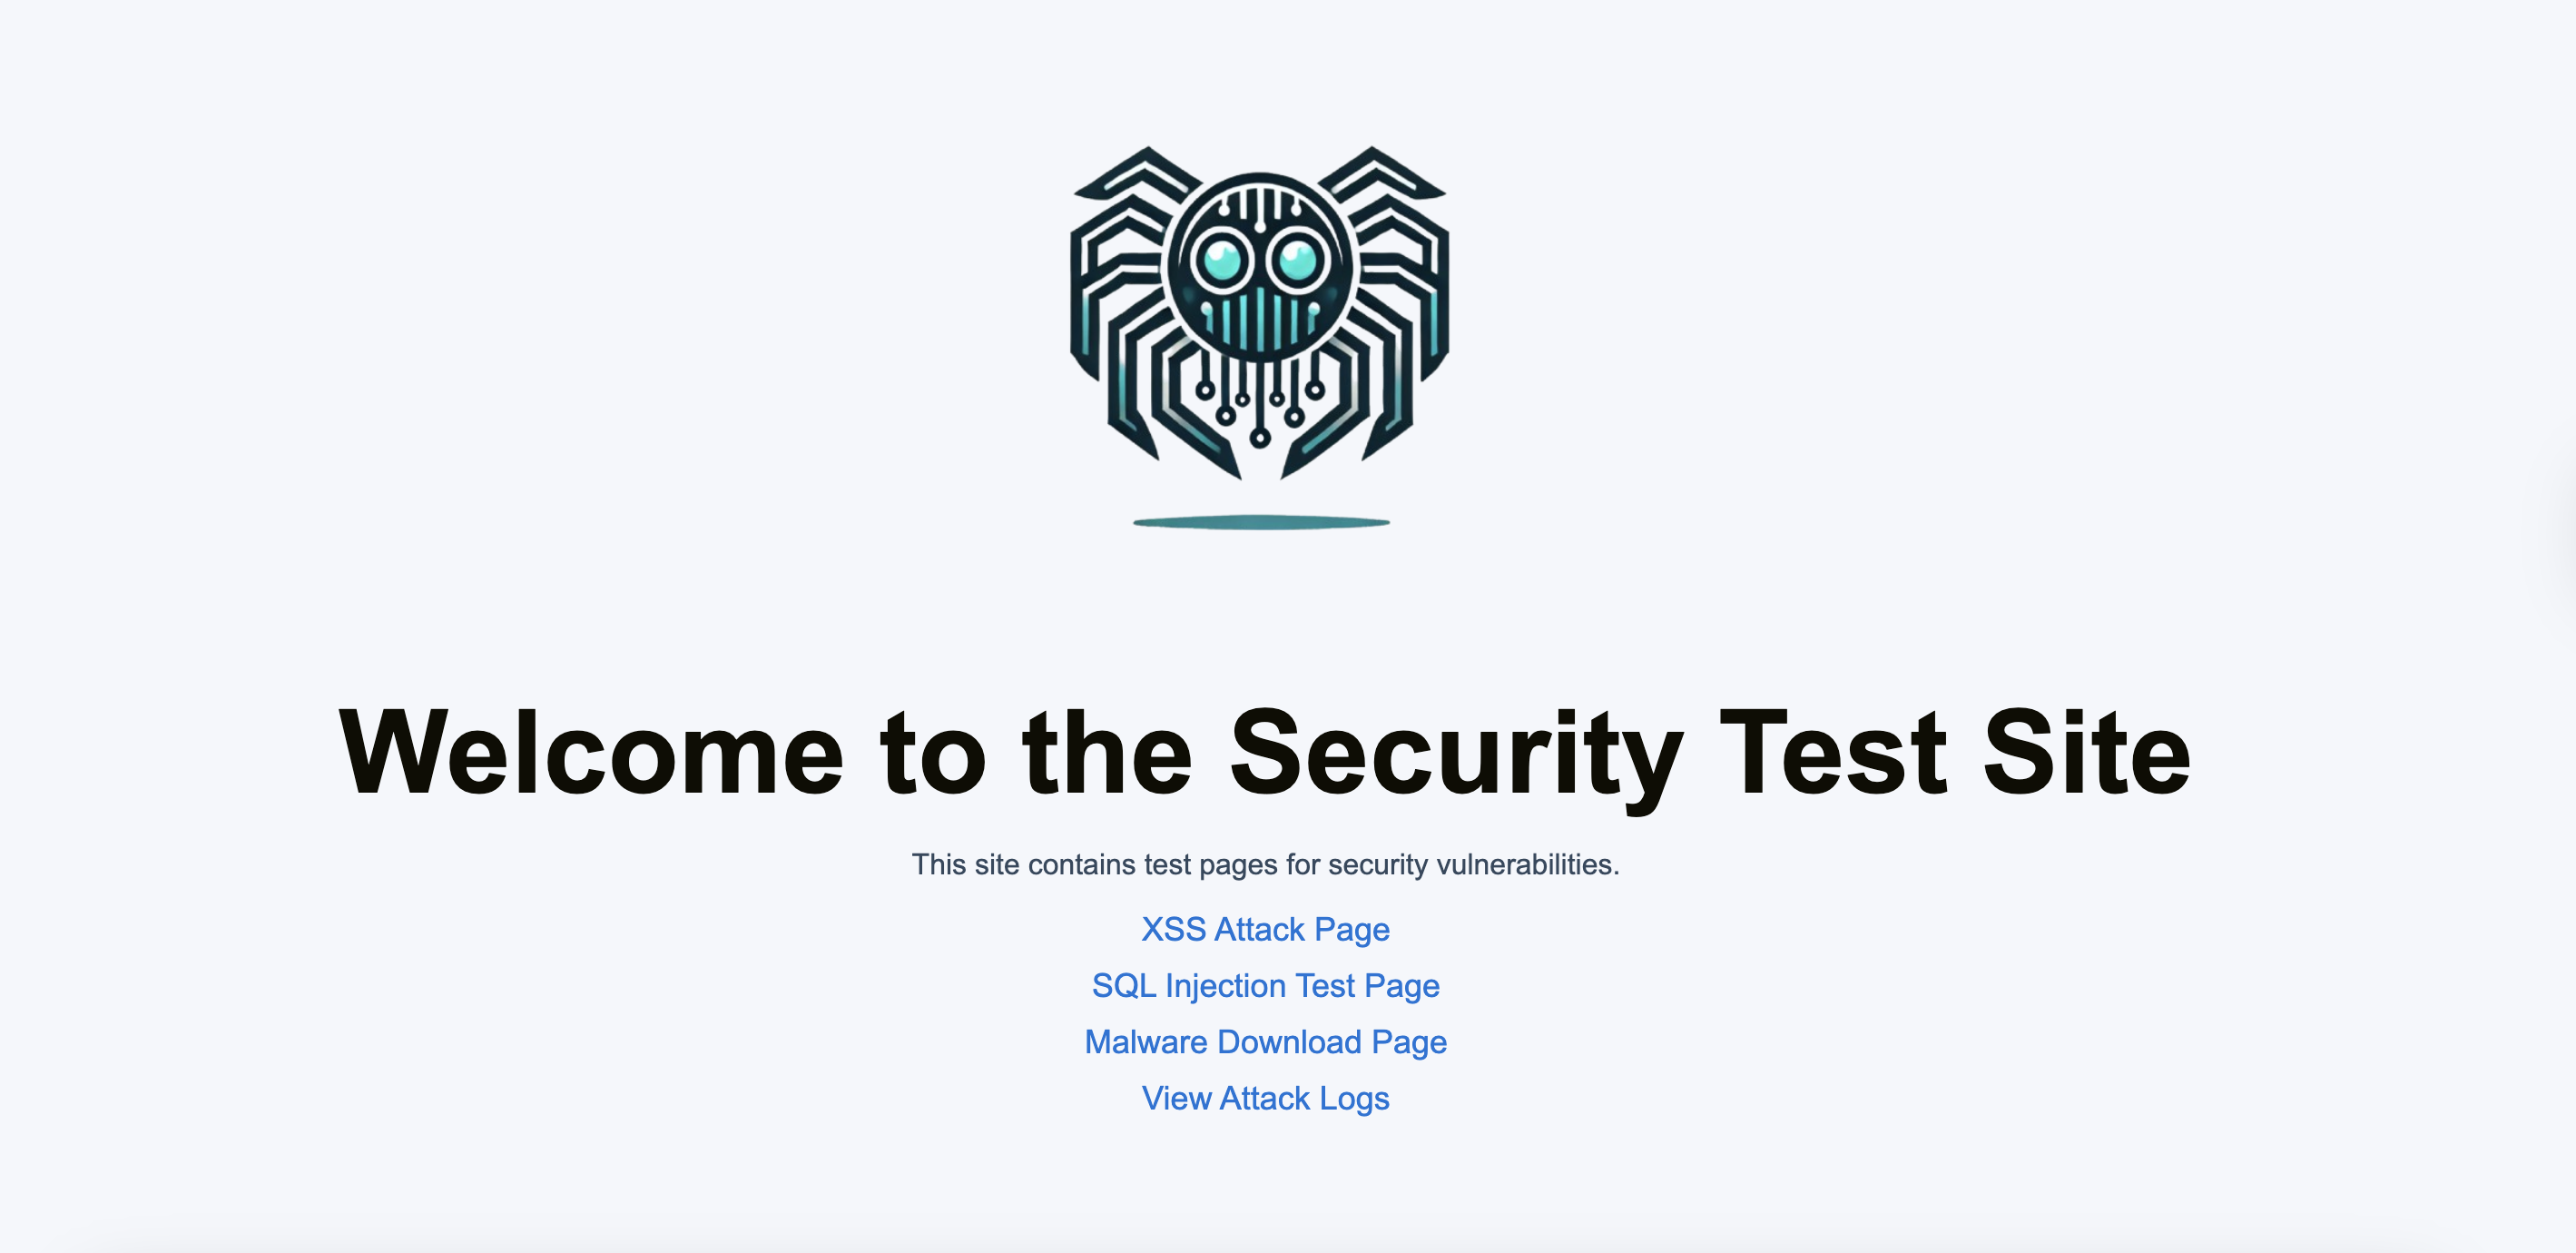
\includegraphics[width=\textwidth]{figures/home.png}
    \caption{Home Page}
    \label{fig:architecture}
    \end{figure*}
    
    \begin{figure*}[!t]
    \centering
    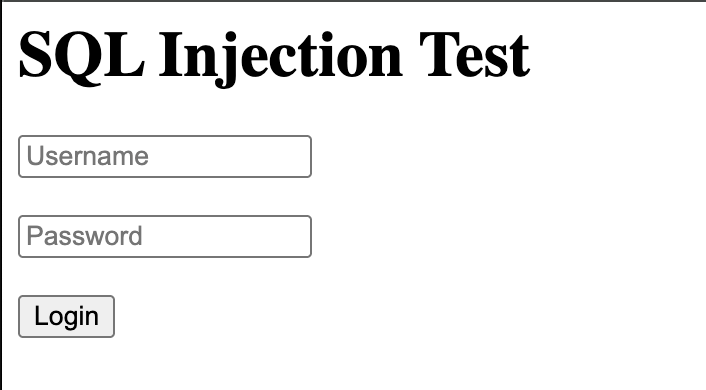
\includegraphics[width=\textwidth]{figures/sqltest.png}
    \caption{SQL Injection Test Site}
    \label{fig:architecture}
    \end{figure*}
    
    \begin{figure*}[!t]
    \centering
    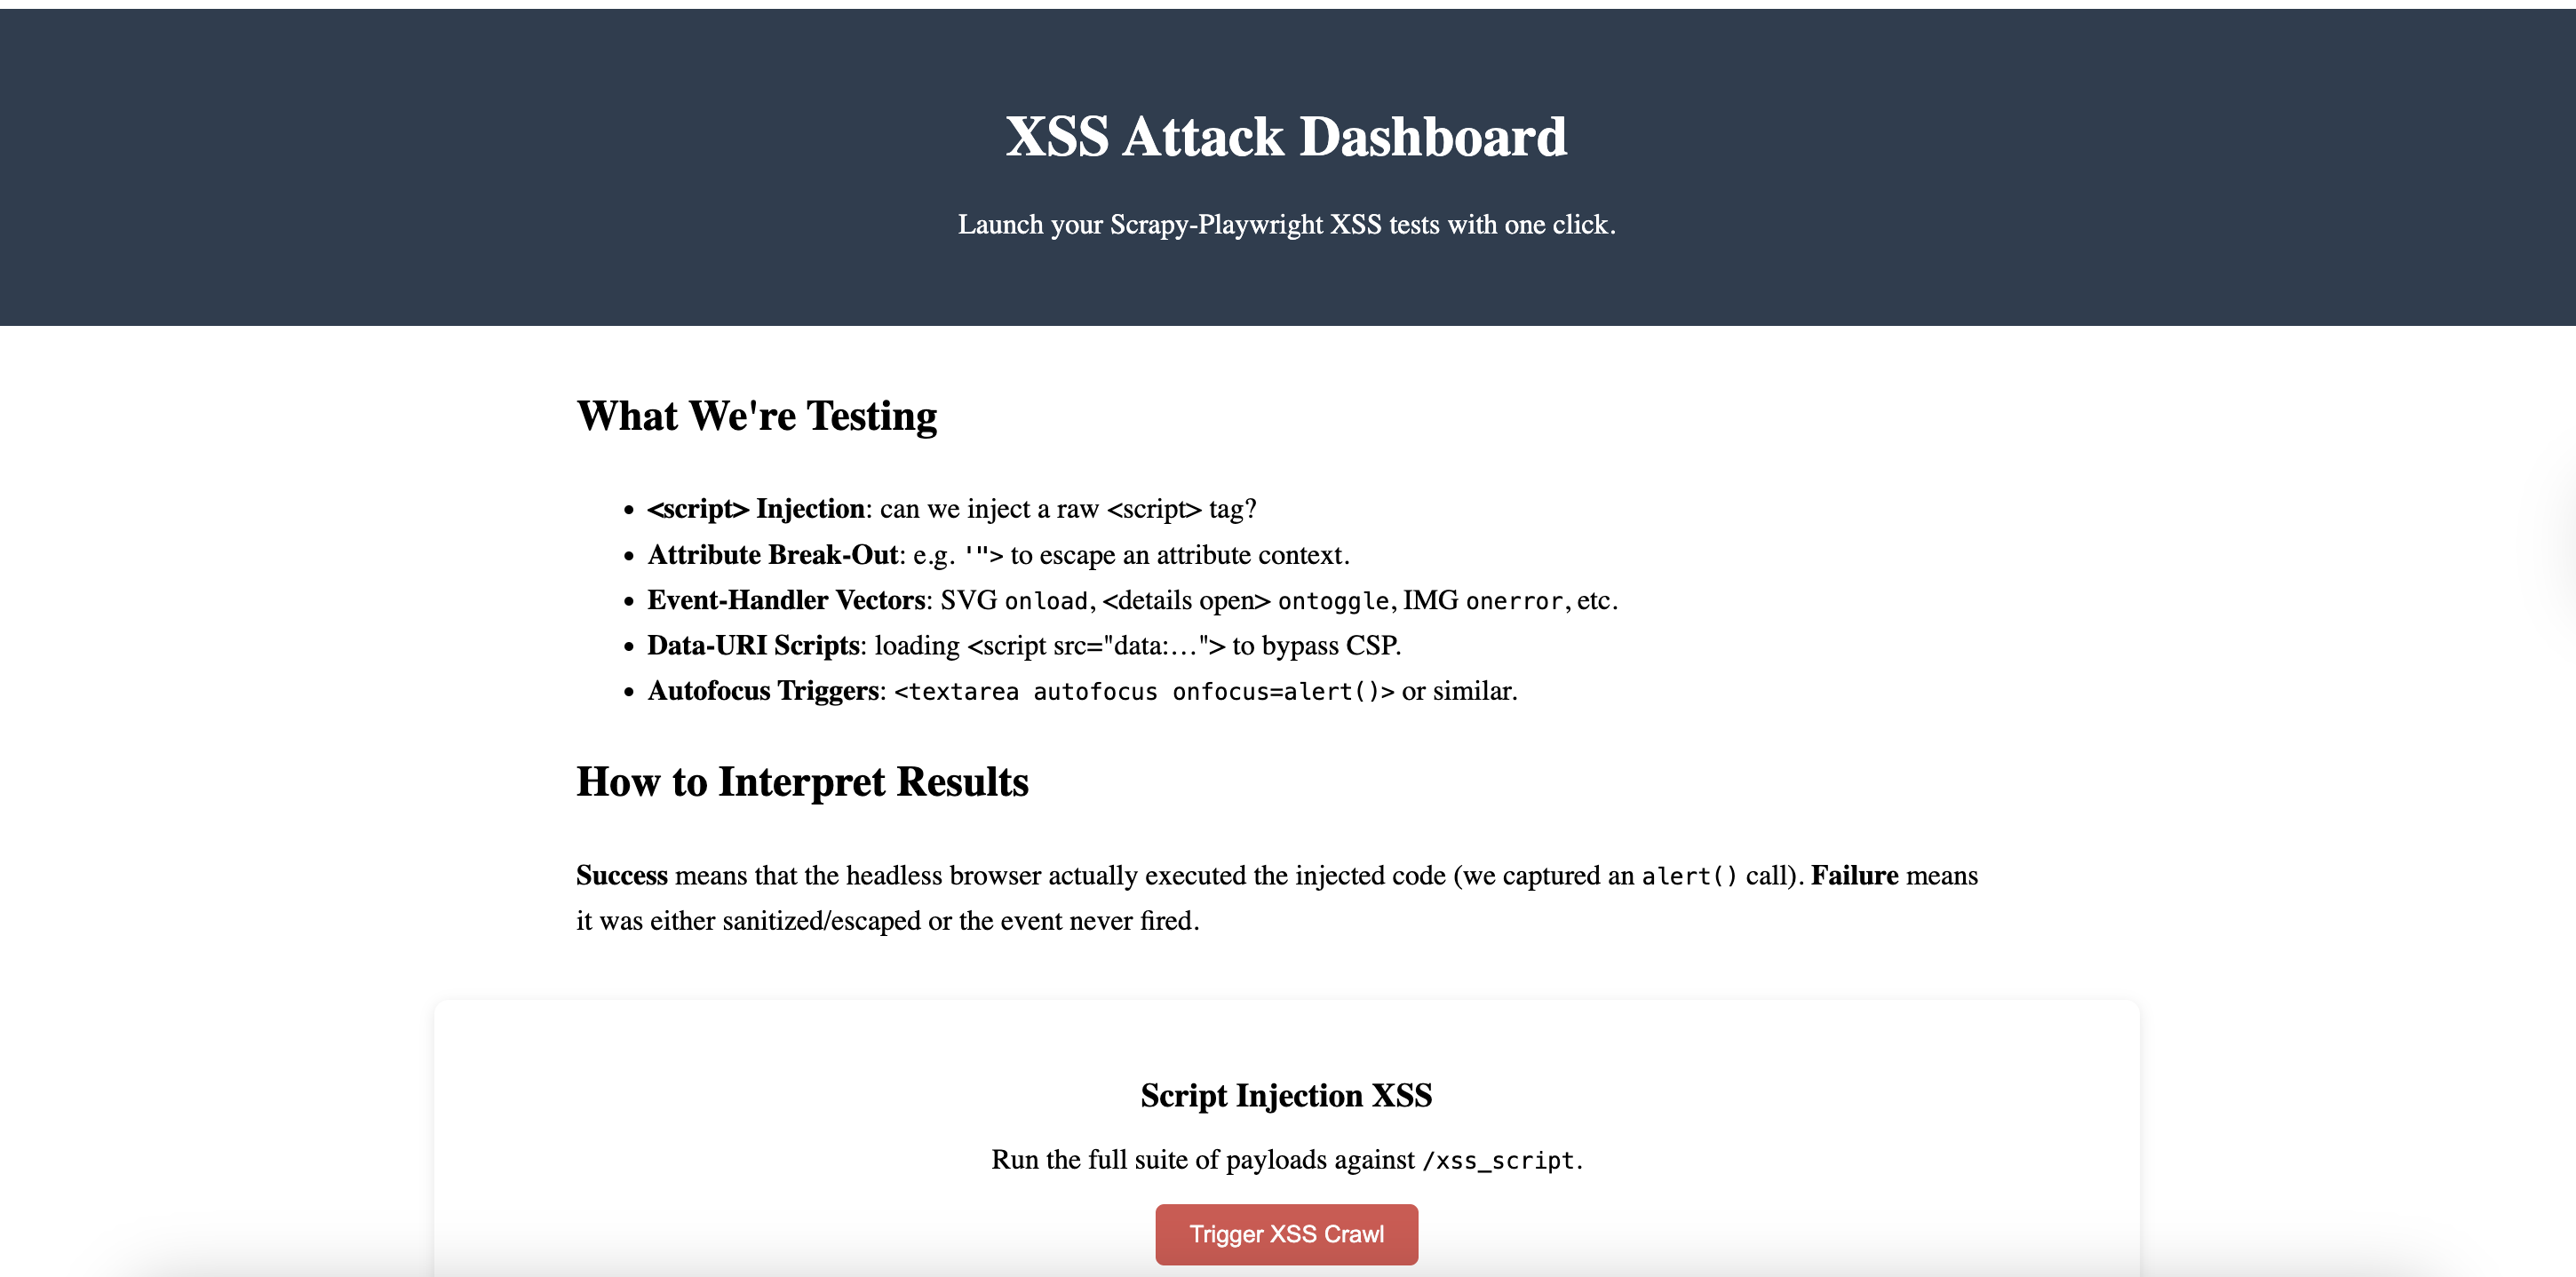
\includegraphics[width=\textwidth]{figures/xssdash.png}
    \caption{XSS Test Site}
    \label{fig:architecture}
    \end{figure*}
    
    \begin{figure*}[!t]
    \centering
    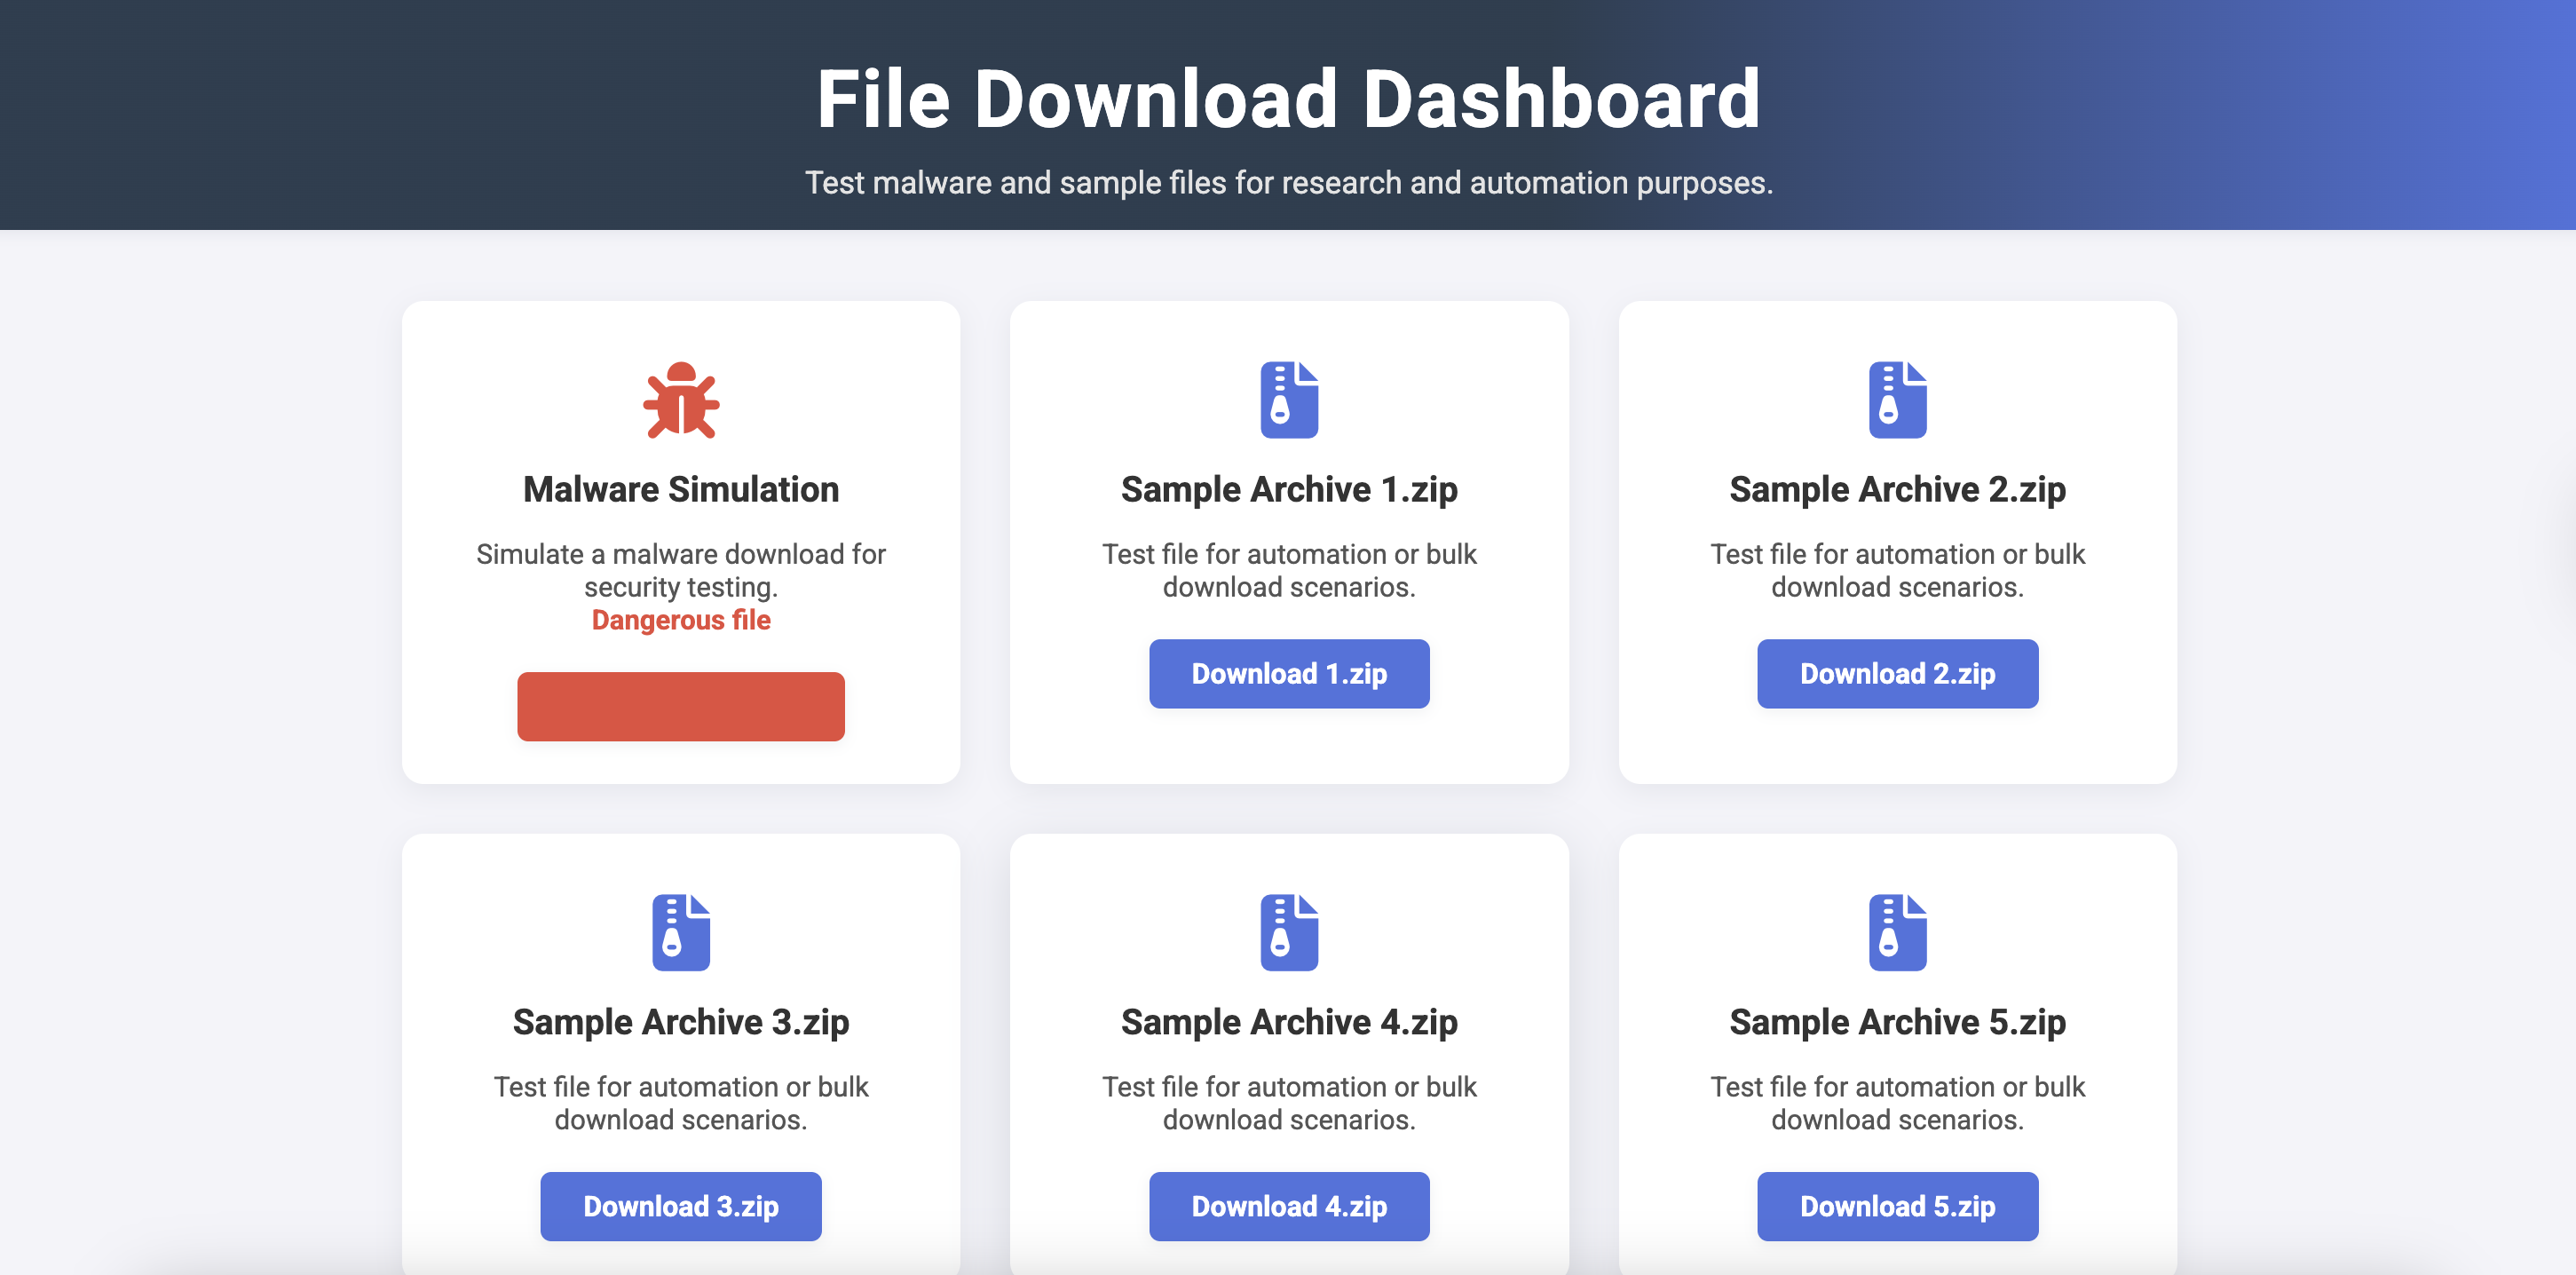
\includegraphics[width=\textwidth]{figures/maldash.png}
    \caption{Malware Download Test Site}
    \label{fig:architecture}
    \end{figure*}
    
  
    \begin{figure*}[!t]
        \centering
        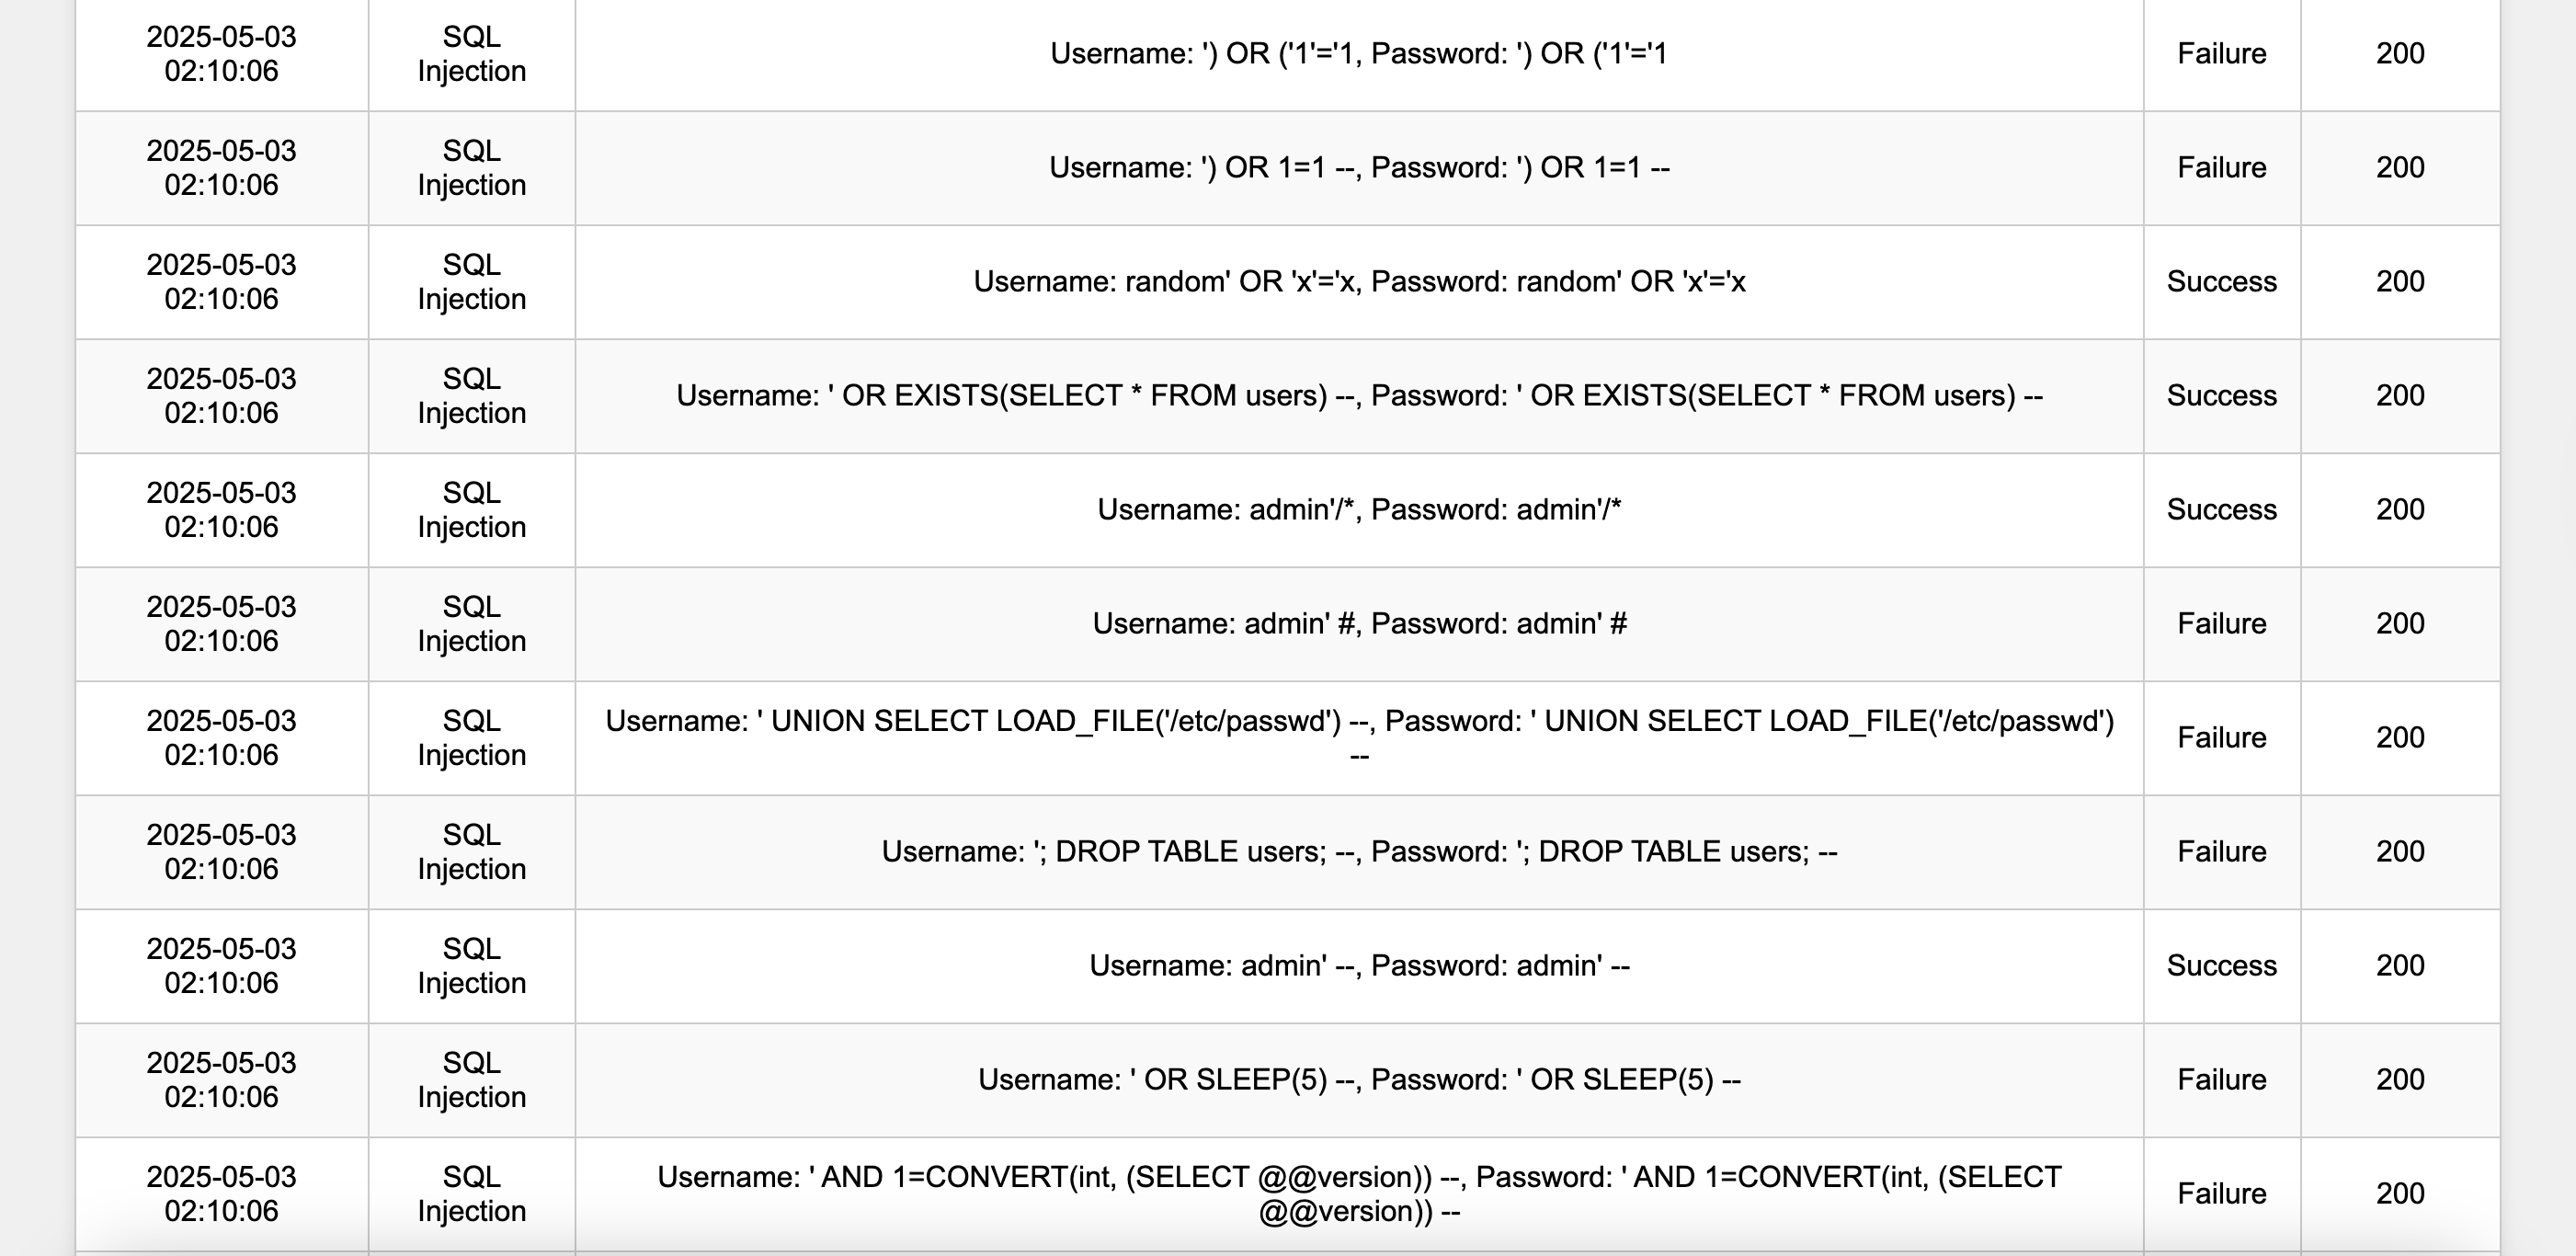
\includegraphics[width=\textwidth]{figures/sqli.png}
        \caption{SQL Injection Results.}
        \label{fig:architecture}
      \end{figure*}
    
      \begin{figure*}[!t]
        \centering
        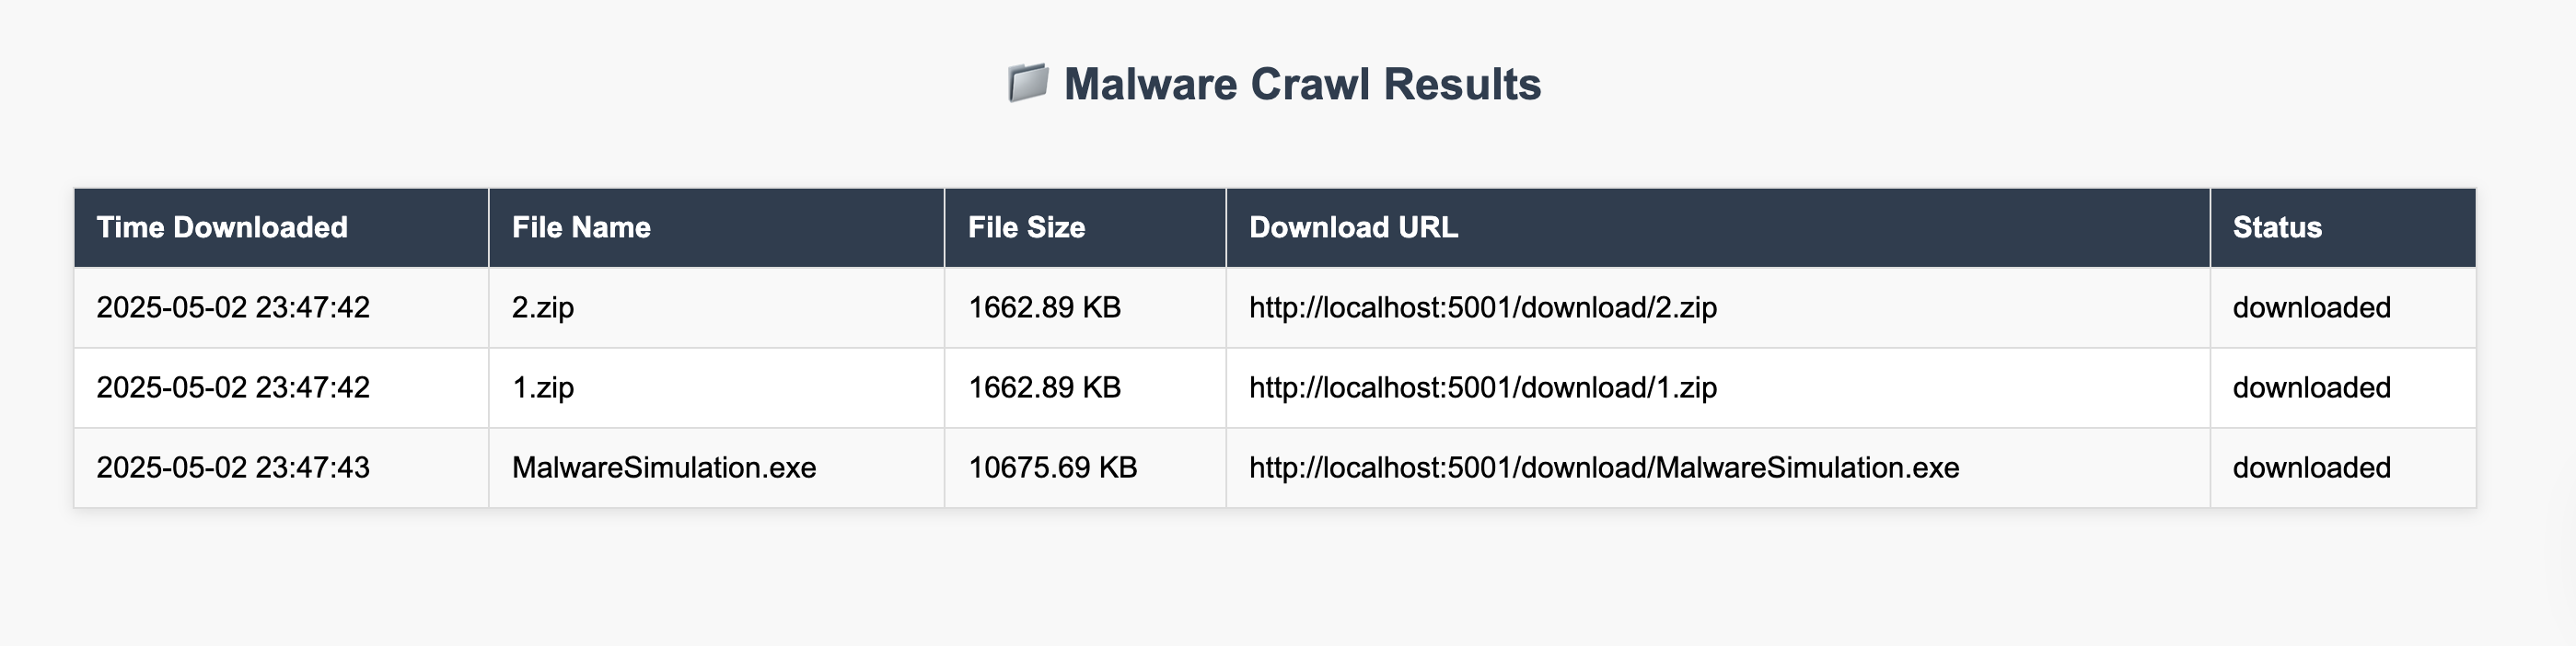
\includegraphics[width=\textwidth]{figures/malres.png}
        \caption{Malware Crawl Results.}
        \label{fig:architecture}
      \end{figure*}